\documentclass{article}

%\documentclass[twocolumn]{article}
%\documentclass{book}
\usepackage{parskip}
\usepackage[bottom=1in]{geometry}
\usepackage{multicol}
\setlength{\columnsep}{0.9cm}
\usepackage{supertabular}
\usepackage[utf8]{inputenc}
%\usepackage{geometry}   % Setup for page and paper dimensions
\usepackage{wrapfig}
\usepackage{subfigure}
\usepackage{caption}
\captionsetup{
  font=small,
  labelfont=bf,
  tableposition=top
}
\usepackage{float}
\usepackage[swedish]{babel}
\usepackage{hyperref}
\hypersetup{
    colorlinks,
    citecolor=black,
    filecolor=black,
    linkcolor=black,
    urlcolor=black,
    pdfborder = {0 0 0}
}
\usepackage{enumitem}
\usepackage{verbatimbox}
\usepackage{fancyvrb}
\usepackage{graphicx}   
\usepackage{lipsum}  
\usepackage[leqno]{amsmath}
\usepackage{listings} 
\usepackage{tikz}
\usepackage{cancel}
\usepackage{steinmetz}
\usepackage{boxdims}

\newcommand*\mycirc[1]{%
\begin{tikzpicture}[baseline={(0,-0.1)}]
\node[draw,circle,inner sep=1pt] {#1};
\end{tikzpicture}}

\newcommand*\textcircle[1]{\textcircled{\raisebox{0.14em}{#1}}}
\newcommand{\quotes}[1]{``#1''}
\usepackage{ifthen}

\makeatletter
\newcommand*{\rom}[1]{\expandafter\@slowromancap\romannumeral #1@}
\makeatother

\usepackage{graphicx}

\makeatletter
\newcommand*\bigcdot{\mathpalette\bigcdot@{.5}}
\newcommand*\bigcdot@[2]{\mathbin{\vcenter{\hbox{\scalebox{#2}{$\m@th#1\bullet$}}}}}
\makeatother

\setlength{\parindent}{0pt}

\newcommand*\sepline{%
  \begin{center}
    \rule[1ex]{.5\textwidth}{.5pt}
  \end{center}}

\newcommand*\sepstars{%
  \begin{center}
    $\star\star\star$
  \end{center}}

\title{lab rf\\}
\author{Lasse Karagiannis}
\date{\today} % Activate to display a given date or no date (if empty),
         % otherwise the current date is printed 
         
\mathchardef\mhyphen="2D

\usepackage{silence}
\WarningFilter{latex}{Underfull}
\WarningFilter{latex}{Overfull}
\WarningFilter{latex}{Text page}
\usepackage{subfiles}



\usepackage{tikz}
\usepackage{tikz}
\usepackage{pgfplots}
\usepgfplotslibrary{smithchart}
\pgfplotsset{compat=1.11}

\newcommand\mtotex[2]{\immediate\write18{m4 #2.m4 | dpic -#1 > #2.tex}}

\begin{filecontents}[overwrite,noheader,nosearch]{sample1.m4}
%\begin{filecontents*}[noheader,force]{sample1.m4}
include(pgf.m4)
.PS
cct_init
elen = 0.75
Origin: Here
source(up_ elen); llabel(-,v_s,+)
resistor(right_ elen); rlabel(,R,)
dot
{  
capacitor(down_ to (Here,Origin))
rlabel(+,v,-);llabel(,C,)
dot
}
line right_ elen*3/3
inductor(down_ Here.y-Origin.y); rlabel(,L,);b_current(i)
line to Origin
.PE
\end{filecontents}

\begin{filecontents}[overwrite,noheader,nosearch]{sample2.m4}
%\begin{filecontents*}[noheader,force]{sample1.m4}
include(pgf.m4)
.PS
cct_init
elen = 0.75
Origin: Here
source(up_ elen,AC); llabel(-,v_s,+)
resistor(right_ elen); rlabel(,R,)
dot
{  

dot
}
line right_ elen*3/3
resistor(down_ Here.y-Origin.y); rlabel(,R,);

line left_ elen*3/3
dot
line to Origin
.PE
\end{filecontents}



\begin{filecontents}[overwrite,noheader,nosearch]{sample3.m4}
%\begin{filecontents*}[noheader,force]{sample1.m4}
include(pgf.m4)
.PS
cct_init
elen = 0.75
Origin: Here
source(up_ elen,AC); llabel(-,v_s,+)
resistor(right_ elen); rlabel(,R,)
dot
{  

dot
}
line right_ elen*1/3
tline(right_ elen);rlabel(,T-line,)
line right_ elen*1/3
dot
line right_ elen*1/3
resistor(down_ Here.y-Origin.y); rlabel(,R,);label(,25,);

line left_ elen*1/3
dot
line left_ elen*5/3
dot
line to Origin
.PE
\end{filecontents}


\begin{filecontents}[overwrite,noheader,nosearch]{sample3A.m4}
include(pgf.m4)
.PS
cct_init
elen = 0.75
Vs: source(up_ elen,AC); llabel(-,v_s,+)
resistor(right_ elen); rlabel(,R_g`\,'50\Omega,) # rlabel sets math mode
D1: dot
#{
#
#dot
#}
line right_ elen*1/3
tline(right_ elen);rlabel(,\hbox{\sl T-line}`\,'50\Omega,)
line right_ elen*1/3
D2: dot
line right_ elen*1/3
resistor(down_ Here.y-Origin.y); rlabel(,R_L,);llabel(,25\Omega,);

#line left_ elen*1/3
#dot
{ dot(at (D1,Here)) }
{ dot(at (D2,Here)) }
#line left_ elen*5/3
line to Vs.start
.PE
\end{filecontents}

\begin{document}

%\begin{titlepage}
%\maketitle
%\end{titlepage}


%\mtotex{g}{sample1}
%\par
%\begin{figure}[ht]
%\input{sample1.tex}
%\caption{customized caption}
%\label{Symbolic_label}
%\end{figure}



%\begin{tikzpicture}
%        \begin{smithchart}
%        \path[draw=red] (0pt,0pt) circle (1.5cm);
%        \path[draw=blue] (0.1,0.5) circle (0.75cm);
%        \path[draw=blue,fill=blue] (0.1,0.5) circle (0.05cm);
%
%       \addplot coordinates {(0.5,0.2) (1,0.8) (2,2)};
%        \end{smithchart}
%    \end{tikzpicture}

\section{ Prerequisites: Installation of QUCS on host}
\begin{multicols}{2}
Downloading the tarballs for QUCS and for
the Verilog-AMS to SPICE-translator ADMS also cloning QUCS  and ADMS from github
in other folders and working on the installation from multiple folders
resulted in many problems related to build process of \verb+qucs-core+.\\

Giving up on the tarball installation folder, I went to the git-clone folder and worked until I gave up and went back again to the
tar-ball folder then gave up and went so back and forth.\\
Errors from not following installation instructions correctly,
errors from uncomplete instructions which assumes a pre-knowledge in
operating system internals (when super-user mode is supposed be used and when not,
the necessity of the setting of enivroment varibles related to \verb+LDPATH+).

Errouneously mixing installation commands for ADMS and for Qucs but also perhaps
because of corruption of tar-balls due to limited and varying internet bandwith.
Read on unix.stackexchange that a certain system administrator often encountered
corrupted tar-balls. Unfourtunately the reference to particular thread is lost but it does not
seem unlikely to me given the fact that the \verb+tar+ command is old and might not have
the same level of sofisticated error correction code as in modern git code,
but I am speaking as layman I don't really know.\\

I also gave up on trying to get the Linux installation to work and tried running the Windows version
``Qucs studio'' on the Wine-platform for Linux but noticed differences in the display compared to
 what was shown in the document ``Getting started with Qucs'' and with Wine having
 the rumor of being buggy I did not dare to proceed. Besides that, I could not
accept defeat from a ``simple'' installation. Done this before.\\

To be honest I don't know for sure why the installation suddenly
worked. Did I finally follow the instructions or was it that the tarballs were corrupted or was it the enivroment variable
or a combination of all these factors?
Cloning the github repositories
did not give the same errors which could be attributed to an possible existence of a check-sum verfification agorithm in git
which possibly is not existing in the \verb+tar+ unpacking command or it could be the case that the build commands
are different  with respect to the git clone installation and therefore caught more attention and care.\\

Posted on Sourceforge\footnote{\url{https://sourceforge.net/p/qucs/discussion/311049/thread/88cc152f64/?limit=25}}
about the build related problems which was ignored because it contained a glaring mistake about the paths provided
where I mixed up \verb+/usr/local/bin+ and \verb+/usr/local/lib+ and also posted another question
on unix.stackexchange \footnote{\url{https://unix.stackexchange.com/questions/715523/what-does-it-mean-when-aclocal-cannot-open-version}}.
related to the Autotools build-tools suite.\\

According to the ADMS section of QUCS on Github \footnote{\url{https://github.com/Qucs/ADMS/blob/develop/README.md}} 
one is supposed to do the following when installing from a tar-ball (which is different from when installing from the github clone)
\begin{verbatim}
tar xvfz adms-x.x.x.tar.gz
cd adms-x.x.x
./configure --prefix=[/install/location/]
make install
\end{verbatim}

The command \verb+make install+ does not work if one is not issuing it as a superuser,
which is implied for those who know but is nowhere written in the instructions so under Linux Ubuntu
one should issue \verb+sudo make install+.
It might be obvious to use super-user mode for someone with who is a complete novice but this is not always true.
In some instances when installing in super-user mode the program is not availible in normal user-mode
and one has to issue a \verb+chmod+ command to allow non super-users access.\\

The descision was for some reason to  install ADMS in the location \verb+/usr/local/lib+ from reading on peoples problems who had
succeeded with the installation on the net. \verb+sudo make install+ returned stating that
the library admsXml could not be found which prompted me to run the configure portion of QUCS as
\verb+./configure --with-mkadms+\\
\verb+=/usr/local/lib/admsXml+ but was still not found or not working.\\
It is also possible that I out of being carless have run 
\verb+./configure --with-mkadms=+\\
\verb+/usr/local/bin/admsXml+ which I stated on the Sourceforge
site thus making a fool of myself.
 The tip using \verb+--with-mkadms+ was not from the official documentation but found
on Stackexchange\footnote{\url{https://stackoverflow.com/questions/36102809/qucs-core-configure-error-needs-admsxml}}.

The ADMS build report which is dispalyed on the terminal during the installation also alludes to that
it in some occations might be necessary to point to \verb+LIBDIR+ but not knowing what \verb+LIBDIR+ was meant to be, I decided to ignore
until I realized that this might be crucial point.\\
Found this discussion on Stackexchange\footnote{\url{https://stackoverflow.com/questions/13428910/how-to-set-the-environmental-variable-ld-library-path-in-linux}}
relating to how to set enivroment varibles in Linux.
I did not do it the official sanctioned Ubuntu way which according to a writer on Stackexchange is the adding of
a \verb+.conf+ file to
\verb+/etc/ld.so.conf.d+ and then in the \verb+.conf+ file write the path to the ADMS-library because it was
not obvious where the  \verb+.conf+ file then should be stored, so I resorted to editing \verb+.bash_profile+
of which I had a vague memory of having done some years ago and it worked then, but not the recommended way according to what someone said on Stackexchange...
Using the rather difficult built in vi-editor \verb+ vi ~/.bash_profile+ the addition was
\begin{verbatim}
LD_LIBRARY_PATH=/usr/local/lib
export LD_LIBRARY_PATH
\end{verbatim}
The \verb+.bash_profile+ which I had edited before was empty when opened and information being lost from there after restart is discussed on mentioned thread
but the work-around suggested results in an error if tried. After editing \verb+.bash_profile+ one is supposed to issue (at the terminal):
\begin{verbatim}
source ~/.bash_profile
sudo ldconfig
\end{verbatim}
Finally, I still could not build the documentation because QUCS uses now obsolete libraries related to TexLive which are
\verb+texlive-math-extra+, and\verb+pgf+. The \verb+pgf+ library is nowhere to be found because it is an instrinsic part of the standard TexLive distribution since years ago.
Luckily QUCS provide the option to not build the documentation using the switch \verb+--disable-doc+ in the top-level configure script.
QUCS also uses an obsololete, at least with respect to Ubuntu, Octave package for converting encapsulated postscript files
\verb+octave-epstk+ which is nowhere to be found except for Debian Linux it seems.\\

Being still at the novice level in installing from source code and not having completed the full verfication of the installation
(\verb+make check+) before throwing out the code folder, the installation is not to be trusted.
 Dr. Dancila helped me with some tests in a Zoom-session
but after the session ended disturbing warnings were detected which were not brought to Dr. Dancila's attention.

\end{multicols}
\section{Verification of the installation with respect to RF-theory and with respect to performance as stated in the QUCS manual}
Doing so many mistakes during the installation there can be no trust that something was not broken or corrupted working
 with both the tarball folder and the git cloned folder for both ADMS and QUCS.
Due to the mistakes during the installation and the many problems encounterd also because of the fact that full built in checks
of the installation were not performed before deleting the code folder, it feels necessary to evaluate the installation with respect to theory
and record warnings and errors for evaluation before proceeding with the lab so to have some level of confidence
that the QUCS installation will actually perform as the authors designed it.
Especially concerning was the following meassage after completing a zoom-session with Dr. Dancila and which was not shown to him.
\begin{verbatim}
Errors and Warnings:
--------------------

line 33: no trailing end-of-line found, continuing...
\end{verbatim}
Does this impact the accuracy of the calculations?
 I certainly would not bet my life on that it does not!\\
Futher more we also want to verify that simple processes which will be used in the lab was not corrupted
such that reading the touchstone file provided by
Dr. Dancila and some of the built in functions which will be used in the lab before actually proceeding to the lab task.
We also repeat the tests done together with the Dr. Dancila for full reference.

\begin{multicols}{2}
The following tests feels suitable to perform at minimum before proceeding with the actual lab-work.
\begin{enumerate}[label=(\alph*)]
\item Reflection coefficient of load without transmission line should be transformed to the correct position in the Smith-chart.
\item Calculation of Return Loss and Mismatch Loss should conform with Matlab/Octave.
\item Reflection coefficient of load with 50 ohm transmission line should be transformed to correct position in the Smith chart
\item Sweeping the length of the transmission line one half wave length shoul result in a plot of the reflection coefficient
describing a full circle.
\item Example 9-13 in David K. Cheng ```Field and wave Electromagnetics''' short circuited line is transformed to a certain
impedance with a transmission line of $0.1\lambda$.
\item Plot of S-parameters verifying that the particular part of the touchstone file is read correctly.
\item Plot of the built in function $Rolett()$ to verify that it accurately performs the calculation of the
Rolett stability condition.
\item Plot of built-in functions $stabL()$ and $stabS()$ verifying input- and output-stability circles with respect to theory.
\item Plot of the Noise-figure data verifying that the particular part of the Touchstone file is read correctly.
\end{enumerate}
\end{multicols}
The Toucstone file is as follows
\begin{verbatim}
! Filename:       BFG520I.S2P       Version:   2.1
! NXP part #: BFG520                                     Date: Feb 1992
! Bias condition: Vce=6V, Ic=10mA
! IN LINE PINNING: same data as with cross emitter pinning.
#  MHz  S  MA  R  50
! Freq       S11            S21            S12            S22     !GUM [dB]
   40    .711  -14.1  23.473  170.8    .007   82.3    .974   -6.8 !    43.5
  100    .690  -34.5  22.218  158.5    .016   74.0    .931  -16.3 !    38.5
  200    .640  -64.3  19.183  141.5    .029   62.4    .816  -28.8 !    32.7
  300    .597  -88.3  16.207  128.8    .037   54.2    .703  -37.1 !    29.1
  400    .569 -106.1  13.627  119.5    .042   50.9    .613  -42.4 !    26.4
  500    .553 -119.9  11.673  112.5    .046   48.6    .544  -45.7 !    24.5
  600    .538 -130.7  10.152  107.0    .050   47.2    .493  -47.6 !    22.8
  700    .526 -139.2   8.947  102.5    .052   47.1    .453  -48.8 !    21.4
  800    .514 -146.7   7.968   98.6    .055   47.9    .422  -49.5 !    20.2
  900    .503 -154.1   7.148   95.1    .057   48.8    .396  -50.2 !    19.1
 1000    .495 -160.2   6.488   92.4    .059   49.7    .374  -51.1 !    18.1
 1200    .494 -171.7   5.468   87.0    .065   51.3    .344  -53.4 !    16.5
 1400    .500 -131.8   4.748   82.0    .069   52.5    .331  -56.1 !    15.3
 1600    .500  173.3   4.159   77.8    .075   55.2    .326  -57.3 !    14.1
 1800    .494  166.0   3.722   74.3    .082   56.4    .317  -57.9 !    13.1
 2000    .496  158.4   3.368   71.0    .087   58.2    .297  -59.5 !    12.2
 2200    .515  151.9   3.080   67.9    .093   59.0    .279  -64.4 !    11.5
 2400    .535  147.6   2.798   64.2    .097   60.7    .280  -71.4 !    10.8
 2600    .540  144.2   2.579   61.6    .107   61.3    .298  -76.3 !    10.1
 2800    .534  139.8   2.428   58.2    .114   60.9    .313  -77.7 !     9.6
 3000    .541  133.9   2.259   55.3    .120   62.3    .309  -78.3 !     9.0
! Noise data:
! Freq.     Fmin        Gamma-opt         rn
  500       1.10     .330     27.0       .250
  900       1.25     .294     48.0       .260
 1000       1.30     .298     52.0       .270
 2000       1.90     .242    134.0       .160

\end{verbatim}
\hspace{1em}\\
\hspace{1em}\\
\hspace{1em}\\
\hspace{1em}\\
\subsection{Tests}
\begin{multicols}{2}
\begin{enumerate}[label=(\alph*)]
\item Reflection coefficient of load without transmission line should be transformed to the correct position in the Smith-chart.\\


When the dimensions of the circuit $d$ are much less than the length of the wavelength $\lambda$ the voltage depends
only on their configuraion in the circuit but geometric distances from the source are of no importance, therefore
sweeping the frequency when there is no difference in the voltage along the line should result in a constant
reflection coefficient for all frequencies.
\mtotex{g}{sample2}
\par
\begin{figure}[H]
%\begin{filecontents*}[noheader,force]{sample1.m4}

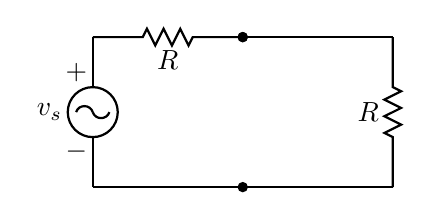
\begin{tikzpicture}[scale=2.54]
% dpic version 2014.Jan.01 option -g for TikZ and PGF 1.01
\ifx\dpiclw\undefined\newdimen\dpiclw\fi
\global\def\dpicdraw{\draw[line width=\dpiclw]}
\global\def\dpicstop{;}
\dpiclw=0.8bp
\dpiclw=0.8bp
\dpicdraw (0,0)
 --(0,0.25)\dpicstop
\dpicdraw (0,0.375) circle (0.049213in)\dpicstop
\dpicdraw (-0,0.375)
 ..controls (-0.013347,0.415042) and (-0.069986,0.415042)
 ..(-0.083333,0.375)\dpicstop
\dpicdraw (0,0.375)
 ..controls (0.013347,0.334958) and (0.069986,0.334958)
 ..(0.083333,0.375)\dpicstop
\dpicdraw (0,0.5)
 --(0,0.75)\dpicstop
\draw (0,0.25) node[below left=-1.5bp]{$ -$};
\draw (-0.125,0.375) node[left=-1.5bp]{$ v_s$};
\draw (0,0.5) node[above left=-1.5bp]{$ +$};
\dpicdraw (0,0.75)
 --(0.25,0.75)
 --(0.270833,0.791667)
 --(0.3125,0.708333)
 --(0.354167,0.791667)
 --(0.395833,0.708333)
 --(0.4375,0.791667)
 --(0.479167,0.708333)
 --(0.5,0.75)
 --(0.75,0.75)\dpicstop
\draw (0.375,0.708333) node[below=-1.5bp]{$ R$};
\dpicdraw[fill=black](0.75,0.75) circle (0.007874in)\dpicstop
\dpicdraw[fill=black](0.75,0.75) circle (0.007874in)\dpicstop
\dpicdraw (0.75,0.75)
 --(1.5,0.75)\dpicstop
\dpicdraw (1.5,0.75)
 --(1.5,0.5)
 --(1.541667,0.479167)
 --(1.458333,0.4375)
 --(1.541667,0.395833)
 --(1.458333,0.354167)
 --(1.541667,0.3125)
 --(1.458333,0.270833)
 --(1.5,0.25)
 --(1.5,0)\dpicstop
\draw (1.458333,0.375) node[left=-1.5bp]{$ R$};
\dpicdraw (1.5,0)
 --(0.75,0)\dpicstop
\dpicdraw[fill=black](0.75,0) circle (0.007874in)\dpicstop
\dpicdraw (0.75,0)
 --(0,0)\dpicstop
\end{tikzpicture}

\caption{When $d<<\lambda$ the dimensions does not impact any behaviour of the circuit}
\label{Symbolic_label}
\end{figure}

The formula for the reflection coefficient $\Gamma$ is
\begin{flalign*}
\Gamma &=\frac{Z_L-Z_0}{Z_L+Z_0}
\end{flalign*}
We are using normalized impedances so the formula is
\begin{flalign*}
\Gamma &=\frac{Z_L/Z_0-1}{Z_L/Z_0+1}\\
       &=\frac{z_L-1}{z_L+1}\\
\end{flalign*}
We recieve
\begin{flalign*}
\Gamma &=\frac{z_L-1}{z_L+1}\\
       &=\frac{25/50-1}{25/50+1}\\
       &=-0.3333
\end{flalign*}
QUCS gives the following results
\begin{figure}[H]
  \includegraphics[width=\linewidth]{A.png}
  \caption{$R=25$ Ohm}
  \label{fig4}
\end{figure}
with no warnings or errors and thus we did not break anything during
the installation here.\\


\item Reflection coefficient of load with 50 ohm transmission
line should be transformed to correct position in the Smith chart\\

\mtotex{g}{sample3A}
\par
\begin{figure}[H]
\input{sample3A.tex}
\caption{When $d<<\lambda$ the dimensions does not impact any behaviour of the circuit}
\label{Symbolic_label}
\end{figure}
If we have $Z_L = 25$ Ohm and 20 mm lossless transmissionline of 50 Ohm applying
a voltage of $2$ GHz, the theory states that the impedance seen at distance
$l$ from the load looking towards the load is
\begin{flalign*}
Z_i &=R_0\frac{Z_L+jR_0tan{\beta l}}{R_0+jZ_Ltan{\beta l}}
\end{flalign*}
What is $\beta l$ ?
$\beta l$ is supposed to be $2\pi l/\lambda$ and we arrive to this because
\begin{flalign*}
\beta &=\omega\sqrt{LC}\hspace{1em}u_p =\frac{1}{\sqrt{LC}}\\
\omega &=2\pi f\hspace{2.3em} u_p =f\lambda\\
\end{flalign*}
So 
\begin{flalign*}
\beta l &= \omega\sqrt{LC}\, l= 2\pi f\sqrt{LC}\, l\\
        &=2\pi\frac{u_p}{\lambda}\sqrt{LC}\, l= 2\pi\frac{1}{\cancel{\sqrt{LC}}\lambda}\cancel{\sqrt{LC}}\, l\\
        &=2\pi l/\lambda
\end{flalign*}
We apparently need a number for $\beta l$ at 2 GHz where $l=1$mm, the wavelength l is
\begin{flalign*}
\lambda &= \frac{u_p}{f} = \frac{3\cdot 10^8}{2\cdot 10^9}=0.15\text{ m} = 150 \text{ mm}
\end{flalign*}
then $l/\lambda$ is
\begin{flalign*}
\frac{l}{\lambda} &= \frac{20}{150}= 0.13333
\end{flalign*}
so
\begin{flalign*}
Z_i &=R_0\frac{Z_L+jR_0tan{\beta l}}{R_0+jZ_Ltan{\beta l}}\\
    &=50\frac{25+j50tan{0.133333}}{50+j25tan{0.13333}}\\
    &=42.677 + 31.832i
\end{flalign*}
Normalized to the transmissionline impedance $Z_i$ becomes $z_i$ as
\begin{flalign*}
z_i&=Z_i/50\\
    &=\frac{42.677 + 31.832i}{50}\\
    &=0.8535 + 0.6366i
\end{flalign*}
To find out which reflection coefficient this represents
we could either calculate $\Gamma$ at the load
and realize that $\Gamma´=\Gamma(z'=20mm)$ is $\Gamma$
measured at the load multiplied with a phase factor $e^{\theta_\gamma}$ 
corresponding to $20$mm or we can simply calculate
\begin{flalign*}
\Gamma_i &=\frac{z_i-1}{z_i+1}
\end{flalign*}
We will do both starting with the last stated equation
\begin{flalign*}
\Gamma_i &=\frac{z_i-1}{z_i+1}\\
         &=\frac{0.8535 + 0.6366i-1}{0.8535 + 0.6366i+1}\\
         &=0.034843 + 0.331507i \\
         &= 0.33\phase{84}^\circ
\end{flalign*}

We also use
We will do both starting with the last stated equation
\begin{flalign*}
\Gamma_i &=\Gamma_Le^{-2\gamma z'}\\
         &=\Gamma_Le^{-j2\beta z'}\\
          &=\Gamma_Le^{-j2\frac{2\pi z'}{\lambda}}\\
          &=\Gamma_Le^{-j2\frac{2\pi 20}{150}}\\  
          &=0.034843 + 0.331507i 
          &= 0.33\phase{84}^\circ       
\end{flalign*}
which is the same result as the first method of calculation.
The last calculations were obtained using the followong Ocatve script
\begin{verbatim}
l=0.020
c = 3E+8
f=2E+9
lambda = c/f
beta=2*pi/lambda
R0=50;
ZL=25;

Zi=R0*((ZL+i*R0*tan(beta*l))...
   /(R0+i*ZL*tan(beta*l)))

zi=Zi/R0

Gamma_i = (zi-1)/(zi+1)

[THETA, R] = cart2pol...
  (real(Gamma_i), imag(Gamma_i))

THETA_GRAD=THETA*180/pi

zL=ZL/R0

Gamma_L = (zL-1)/(zL+1)
Gamma_i2 = Gamma_L*exp(-i*2*beta*l)

\end{verbatim}

The QUCS installation also gives the same
results. We also notice that the point seems to be correct
located on the Smith Chart which is almost straight
above the centerpoint of the Smithchart $(1,0)$.
\begin{figure}[H]
  \includegraphics[width=\linewidth]{tline1.png}
  \caption{$R=25$ Ohm, 20 mm 50 Ohm transmissionline}
  \label{fig4}
\end{figure}
It is easier to verify the correctness of the point if
the length of the line is swept from 0 to 20 mm so that ones
sees on the Smithchart how the reflection coefficient changes when
the length of the transmissionline varies.
We expect to see a clockwise arc.
\begin{figure}[H]
  \includegraphics[width=\linewidth]{tline2.png}\setcounter{enumi}{4}
  \caption{Clockwise rotation of $\Gamma$ is ``Towards the generator''}
  \label{fig4}
\end{figure}
with no warnings or errors and thus we did not break anything during
the installation here but we found the transient simulation to be
broken.
\begin{figure}[H]
  \includegraphics[width=\linewidth]{tline3.png}
  \caption{Transient simulation is broken}
  \label{fig4}
\end{figure}

\item Calculation of Return Loss and Mismatch Loss should conform with Matlab/Octave.

Here it looks like that QUCS is broken. The result does not conform with Matlab/Octave
\begin{figure}[H]
  \includegraphics[width=\linewidth]{tline4.png}
  \caption{log-calculations are rubbish. Installation is broken}
  \label{fig4}
\end{figure}

Octave gives the following Return Loss
\begin{figure}[H]
  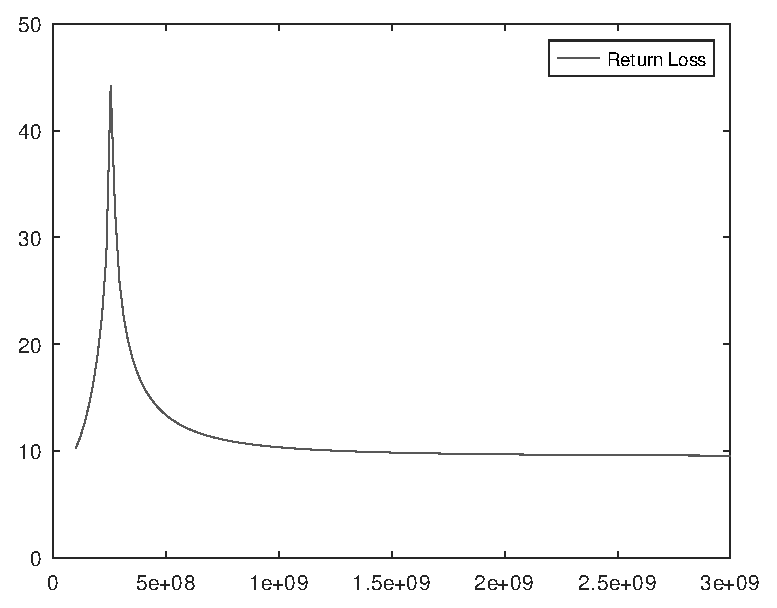
\includegraphics[width=\linewidth]{return_loss.eps}
  \caption{Return Loss}
  \label{fig4}
\end{figure}
and the following Mismatch Loss
\begin{figure}[H]
  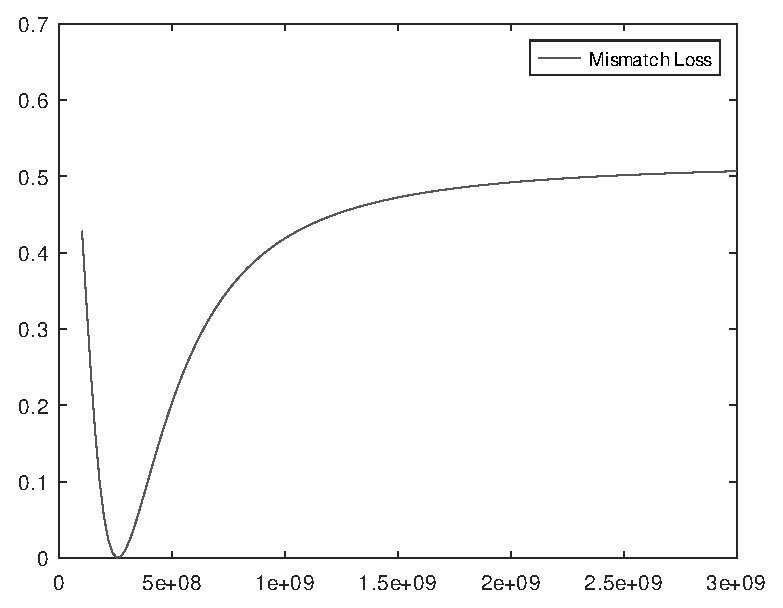
\includegraphics[width=\linewidth]{mismatch_loss.eps}
  \caption{Mismatch Loss}
  \label{fig4}
\end{figure}
From the following Octave code
\begin{verbatim}
l=0.020
c = 3E+8
f_start=0.1E+9;
f_stop=3.0E+9;
n_steps = 150;
step_size=(f_stop-f_start)/n_steps;
f=f_start:step_size:f_stop
GammaIn =zeros(size(f));

R0=50;
ZL=25;

for i=1:n_steps+1
      lambda = c/f(i)
      beta=2*pi/lambda

      Zi=R0*((ZL+i*R0*tan(beta*l))...
         /(R0+i*ZL*tan(beta*l)))

      zi=Zi/R0

      Gamma_i = (zi-1)/(zi+1);
      GammaIn(i)=Gamma_i;

 endfor

RL = -20*log10(abs(GammaIn));

ML = -10*log10(1-abs(GammaIn).^2);
figure(1)
plot(f,RL,";Return Loss;");

figure(2)
plot(f, ML, ";Mismatch Loss;")

\end{verbatim}


\item Sweeping the length of the transmission line one half wave length shoul result in a plot of the reflection coefficient
describing a full circle.

If we apply 3 GHz we will have a wave length of 100 mm, so sweeping the length of the transmission line from 0 mm to
$\lambda/2 = 50$mm must result in a full circle drawn in clockwise direction.
 Here we sweep to 75\% of $\lambda/2$ to verify that the circle grows clockwise ``towards the generator''.
\begin{figure}[H]
  \includegraphics[width=\linewidth]{tline5.png}
  \caption{Sweeping the lenght of the transmission line from 0 mm to 75\% of $\lambda/2$}
  \label{fig4}
\end{figure}

\item Example 9-13 in David K. Cheng ```Field and wave Electromagnetics''' short circuited line is transformed to a certain
impedance with a transmission line of $0.1\lambda$.

The example states - use the Smith chart to find the imput impedance of a section of 50 $\Omega$ lossless transmission
line that is 0.1 wavelength long and is terminated in a short circuit.

The formula for the input impedance is
\begin{flalign*}
Z_i &=R_0\frac{Z_L+jR_0tan{\beta l}}{R_0+jZ_Ltan{\beta l}}
\end{flalign*}
and setting $Z_L = 0$  and $l= 0.1\lambda $ gives
\begin{flalign*}
Z_i &=R_0\frac{0+jR_0tan{\beta l}}{R_0+j\cdot 0\cdot tan{\beta l}}\\
    &=jR_0tan{\beta l} = jR_0tan{2\pi\cdot 0.1}\\
    &= 0 + 36.3271i
\end{flalign*}
which means that the normalized impedance $z_i=i0.726542528$
The corresponding reflection coefficient should read
\begin{flalign*}
\Gamma_i &=\frac{z_1-1}{z_1+1}\\
         &=-0.3090 + 0.9511i
\end{flalign*}
Which also conforms to the QUCS calculation
\begin{figure}[H]
  \includegraphics[width=\linewidth]{tline6.png}
  \caption{Sweeping the lenght of shortcircuited transmission line from 0 mm to 10mm at 3GHz}
  \label{fig4}
\end{figure}

\item Plot of S-parameters verifying that the particular part of the touchstone file is read correctly.

The reading is correct
\begin{figure}[H]
  \includegraphics[width=\linewidth]{tline7.png}
  \caption{S-parameter sweep with excerpt of .s2p-file at 1GHz}
  \label{fig4}
\end{figure}
though errors were detected by the simulator according to the log
\begin{verbatim}
Errors occurred during simulation
on sön 04. sep 2022 at 22:19:18:426
Aborted.



Errors and Warnings:
--------------------

checker error, no actions defined: nothing to do

\end{verbatim}

\item Plot of the built in function $Rollet()$ to verify that it accurately performs the calculation of the
Rollet stability condition.

We notice that the transistor is unstable for low frequencies ($K<1$)
Looks  the same as the one calculated in Matlab
\begin{figure}[H]
  \includegraphics[width=\linewidth]{tline8.png}
  \caption{Rollet stability factor K}
  \label{fig4}
\end{figure}

\begin{figure}[H]
  \includegraphics[width=\linewidth]{K.eps}
  \caption{Rollet stability factor K calculated with Matlab}
  \label{fig4}
\end{figure}
Cleand the .s2p file of the comments and the noisefigeure data and adapted 
code from Mathworks\footnote{\url{https://se.mathworks.com/matlabcentral/answers/76197-how-to-read-strings-from-file-with-fscanf-or-sscanf-not-textscan}}
\begin{verbatim}
fid  = fopen('Spar.s2p', 'r') ;
 data = cell(1e6, 9) ;       % Prealloc.
 rCnt = 0 ;                  % Row counter.
 while ~feof(fid)
    rCnt = rCnt + 1 ;
    data{rCnt,1} = fscanf(fid, '%f', 1);
    data{rCnt,2} = fscanf(fid, '%f', 1);
    data{rCnt,3} = fscanf(fid, '%f', 1);
    data{rCnt,4} = fscanf(fid, '%f', 1);
    data{rCnt,5} = fscanf(fid, '%f', 1);
    data{rCnt,6} = fscanf(fid, '%f', 1);
    data{rCnt,7} = fscanf(fid, '%f', 1);
    data{rCnt,8} = fscanf(fid, '%f', 1);
    data{rCnt,9} = fscanf(fid, '%f', 1);
 end
 fclose(fid) ;
 data = data(1:rCnt,:) ;   % Truncate.
A=cell2mat(data);
f=A(:,1);
S11=zeros(size(f))
S21=zeros(size(f))
S12=zeros(size(f))
S22=zeros(size(f))
j=sqrt(-1);
for i=1:size(f)
 phi = deg2rad(A(i,3))
 phi1 = A(i,3)*pi/180
 S11(i)=A(i,2)*(cos(phi)+j*sin(phi))
 phi= deg2rad(A(i,5))
 S21(i)=A(i,4)*(cos(phi)+j*sin(phi))
 phi= deg2rad(A(i,7))
 S12(i)=A(i,6)*(cos(phi)+j*sin(phi))
 phi= deg2rad(A(i,9))
 S22(i)=A(i,8)*(cos(phi)+j*sin(phi))
end
Delta = abs(S11.*S22-S12.*S21)
K=(1-abs(S11).^2-abs(S22).^2+abs(Delta).^2)...
  ./(2*abs(S12.*S21))
plot(f,K)
legend('K')
\end{verbatim}
\end{enumerate}
\end{multicols}
\begin{enumerate}[label=(\alph*)]
\setcounter{enumi}{9}
\item Plot of built-in functions $stabL()$ and $stabS()$ 
verifying input- and output-stability circles with respect to theory.
\begin{figure}[H]
  \includegraphics[width=\linewidth]{tline9.png}
  \caption{Input and output stability circles}
 \label{fig4}
\end{figure}
\end{enumerate}
%100 MHz;200 MHz;300 MHz;400 MHz;500 MHz;600 MHz;700 MHz;800 MHz;900 MHz;1 GHz;1.2 GHz;1.4GHz;1.6 GHz;1.8 GHz;2.0 GHz;2.2 GHz;2.4 GHz;2.6 GHz;2.8 GHz;3.0 GHz




\section{Amplifier Theory, Chap. 12 in Pozar}
In this section we will verify the equations presented in Pozar in the chapter about Microwave amplifiers.
Pozar posts the following figure
\begin{figure}[H]
 \includegraphics[width=\linewidth]{Pozar1.png}
  \caption{Pozar figure Chap. 12}
  \label{fig4}
\end{figure}
\begin{multicols}{2}
\subsection{$\Gamma_L$ and $\Gamma_S$}
Pozar starts with the presentation of standard well known basic Electromagnetic Theory of
the load reflection coefficient $\Gamma_L$
\begin{flalign*}
\Gamma_L &= \frac{Z_L-Z_0}{Z_L+Z_0}
\end{flalign*}
The source reflection coefficient looking into the load
\begin{flalign*}
\Gamma_S &= \frac{Z_S-Z_0}{Z_S+Z_0}
\end{flalign*}
Then he defines voltage scattering parameters which according to what I've seen differ between authors.
\begin{flalign*}
V_1^- &=S_{11}V_1^+ +S_{12}V_2^+\\
V_2^- &=S_{21}V_1^+ +S_{22}V_2^+\\
\end{flalign*}
This definition is apparently only valid when the source resistor and the load is equal
to the characteristic impedance\footnote{\url{https://en.wikipedia.org/wiki/Scattering_parameters}}
and is in its general way defined as
\begin{flalign*}
b_1 &=S_{11}a_1 +S_{12}a_2\\
b_2&=S_{21}a_1 +S_{22}a_2\\
\end{flalign*}
where 
\begin{flalign*}
a&=\frac{1}{2}\frac{V+Z_oI}{\sqrt{|Re(Z_0)|}}\\
b&=\frac{1}{2}\frac{V+Z_o^*I}{\sqrt{|Re(Z_0)|}}\\
\end{flalign*}
See footnote\footnote{\url{https://se.mathworks.com/discovery/s-parameter.html}}.
It is unclear how one arrives at the Pozar expression of the scattering parameters from the general
definition and for now will not try to show this.
We think it is very unfourtunate that Pozar does not show this.

Since the load voltage coefficient $\Gamma_L$, looking into the load is the quotient between the backward travelling wave $V_2^+$
and the forward travelling wave $V_2^-$, which is 
\begin{flalign*}
\Gamma_L&=\frac{V_2^+}{V_2^-}
\end{flalign*}
and the source reflection coefficient $\Gamma_S$ looking into the generator also is the backward wave (to the load) divided
with the forward wave (into the generator)
\begin{flalign*}
\Gamma_S&=\frac{V_1^+}{V_1^-}
\end{flalign*}
Pozar rewrites equation $(1)$ where he replaces $V_2^+$ with $\Gamma_L V_2^-$
\begin{flalign*}
V_1^- &=S_{11}V_1^+ +S_{12}\Gamma_L V_2^-&(1)\\
V_2^- &=S_{21}V_1^+ +S_{22}\Gamma_L V_2^-&(2)\\
\end{flalign*}
\end{multicols}

\subsection{$\Gamma_{in}$ -Reflection coefficient looking into the network }
\begin{multicols}{2}
Pozar arrives at $\Gamma_{in}$ the reflection coefficient looking into the network, which
is the backward wave divided with the forward wave.
\begin{flalign*}
\Gamma_{in}&=\frac{V_1^-}{V_1^+}
\end{flalign*}

and finds an expression for $\Gamma_{in}$ as a function of the S-parameters by solving for $V_2^-$ in equation 
$(1)$ and inserting it into equation $(2)$ and then solving for the quotient $\frac{V_1^-}{V_1^+}$ thus
obtaining a new expression for $\Gamma_{in}$
\begin{flalign*}
V_1^- &=S_{11}V_1^+ +S_{12}\Gamma_L V_2^-\iff\\
V_2^- &=\frac{V_1^- -S_{11}V_1^+}{S_{12}\Gamma_L }
\end{flalign*}
Inserting the expression of $V_2^-$ into $(2)$ gives
\begin{flalign*}
V_2^- &=S_{21}V_1^+ +S_{22}\Gamma_L V_2^-&(2)\\
\frac{V_1^- -S_{11}V_1^+}{S_{12}\Gamma_L }&=S_{21}V_1^+ +S_{22}\Gamma_L \frac{V_1^- -S_{11}V_1^+}{S_{12}\Gamma_L }
\end{flalign*}
We collect the terms with $V_1^-$ to the left and the terms with $V_1^+$ to the right but first
we clean the denominator on the left hand side
\begin{flalign*}
V_1^- -S_{11}V_1^+&=S_{12}\Gamma_L S_{21}V_1^+ \\
                 &\hspace{1em}+S_{12}\Gamma_L S_{22}\Gamma_L \frac{V_1^- -S_{11}V_1^+}{S_{12}\Gamma_L }
\end{flalign*}
We see that $S_{12}\Gamma_L$ cancels up and down on the second term of the right hand side
\begin{flalign*}
V_1^- -S_{11}V_1^+&=S_{12}\Gamma_L S_{21}V_1^+ \\
                 &\hspace{1em}+ S_{22}\Gamma_LV_1^- -S_{22}\Gamma_LS_{11}V_1^+
\end{flalign*}
Now we are ready to collect the terms with $V_1^-$ and $V_1^+$ left and right
\begin{flalign*}
V_1^- - S_{22}\Gamma_LV_1^-&=S_{11}V_1^+ +S_{12}\Gamma_L S_{21}V_1^+  \\
                           &\hspace{1em}-S_{22}\Gamma_LS_{11}V_1^+
\end{flalign*}
We break out 
\begin{flalign*}
V_1^-(1 - S_{22}\Gamma_L)&=V_1^+(S_{11} +S_{12}\Gamma_L S_{21}-S_{22}\Gamma_LS_{11})
\end{flalign*}
and solve for $V_1^- /V_1^+ $
\begin{flalign*}
\frac{V_1^-}{V_1^+}&=\frac{S_{11} +S_{12}\Gamma_L S_{21}-S_{22}\Gamma_LS_{11}}{1 - S_{22}\Gamma_L}
\end{flalign*}
This does not look like Pozar's expression but if we break out $S_{11}$ from the numerator we get
\begin{flalign*}
\frac{V_1^-}{V_1^+}&=\frac{S_{11}(1-S_{22}\Gamma_L) +S_{12}\Gamma_L S_{21}}{1 - S_{22}\Gamma_L}
\end{flalign*}
and we write the right hand side as two terms
\begin{flalign*}
\frac{V_1^-}{V_1^+}&=\frac{S_{11}(1-S_{22}\Gamma_L)}{1 - S_{22}\Gamma_L} +\frac{S_{12}\Gamma_L S_{21}}{1 - S_{22}\Gamma_L}
\end{flalign*}
Now we see that a common term is cancelled up and down at the first term on the right hand side and we arrive at
Pozar's expression
\begin{flalign*}
\frac{V_1^-}{V_1^+}&=S_{11} +\frac{S_{12} S_{21}\Gamma_L}{1 - S_{22}\Gamma_L}
\end{flalign*}
Thus Pozar arrived at an expression for $\Gamma_{in}$ only involving S-parameters and $\Gamma_L$
\begin{flalign*}
\Gamma_{in}=\frac{V_1^-}{V_1^+}&=S_{11} +\frac{S_{12} S_{21}\Gamma_L}{1 - S_{22}\Gamma_L}
\end{flalign*}
\end{multicols}
\subsection{$\Gamma_{out}$ -Reflection coefficient looking into the network from the load side}
\begin{multicols}{2}
Obviously $\Gamma_{out}$ looking into the network from the load side must be (by symmetry)
\begin{flalign*}
\Gamma_{out}=\frac{V_2^-}{V_2^+}&=S_{22} +\frac{S_{12} S_{21}\Gamma_S}{1 - S_{11}\Gamma_S}
\end{flalign*}
which Pozar also states without evidence, but we can show this also for completeness.

The reflection coefficient looking into the source $\Gamma_S$ having the network at the back is
the backward moving wave $V_1^+$ going into the network divided by the forward going wave travelling
into the source $V_1^-$
\begin{flalign*}
\Gamma_{S}&=\frac{V_1^+}{V_1^-}\iff\\
V_1^+ &=\Gamma_SV_1^-\\
\end{flalign*}
which means that we can re-write Pozar's S-parameter definition
\begin{flalign*}
V_1^- &=S_{11}V_1^+ +S_{12}V_2^+\\
V_2^- &=S_{21}V_1^+ +S_{22}V_2^+\\
\end{flalign*}
as
\begin{flalign*}
V_1^- &=S_{11}\Gamma_SV_1^- +S_{12}V_2^+\\
V_2^- &=S_{21}\Gamma_SV_1^- +S_{22}V_2^+\\
\end{flalign*}
We are hunting for the expression $\Gamma_{out}$ looking into the network from the load side so we
obviously must solve for $V_1^-$ from the first equation above and insert it into the second
\begin{flalign*}
V_1^- &=S_{11}\Gamma_SV_1^- +S_{12}V_2^+\iff\\
V_1^-(1-S_{11}\Gamma_S)&=S_{12}V_2^+\iff\\
V_1^-&=\frac{S_{12}V_2^+}{1-S_{11}\Gamma_S}
\end{flalign*}
Inserting the expression of $V_1^-$ into the second equations
\begin{flalign*}
V_2^- &=S_{21}\Gamma_SV_1^- +S_{22}V_2^+\\
      &=S_{21}\Gamma_S\frac{S_{12}V_2^+}{1-S_{11}\Gamma_S} +S_{22}V_2^+\\
\end{flalign*}
Solving for $V_2^-/V_2^+$
\begin{flalign*}
\frac{V_2^-}{V_2^+} &=S_{21}\Gamma_S\frac{S_{12}}{1-S_{11}\Gamma_S} +S_{22}\\
\end{flalign*}
Which is the wanted expression if we just write it in order
\begin{flalign*}
\Gamma_{out}=\frac{V_2^-}{V_2^+} &=S_{22}+\frac{S_{12}S_{21}\Gamma_S}{1-S_{11}\Gamma_S}\\
\end{flalign*}
\end{multicols}

\subsection{Availible power to the network $P_{in}$}
Pozar want to derive an expression for the power gain $G=P_L/P_{in}$ further down the road. It is is the quotient of the power
delivered to the load to the power availible to the network.
Pozar is not clear, I thought that he wanted to establish a power-wave
\begin{flalign*}
P_{in} &=\frac{1}{Z_0}\frac{V_1^+}{\sqrt{2}}\frac{V_1^{+*}}{\sqrt{2}}\\
       &=\frac{1}{2Z_0}|V_1^+|^2\\
\end{flalign*}
but this is not the case. He defines $P_{in}$ as
\begin{flalign*}
P_{in} &=\frac{1}{2Z_0}V_1\cdot V_1^*
\end{flalign*}
where the factor an half comes from scaling to effective values.

He starts with
establishing that the voltage $V_1 = V_1^+ +V_1^-$ is simply the voltage divder expression
Because
\begin{flalign*}
V_1 &=V_S\frac{Z_{in}}{Z_{in} + Z_S}=V_1^+ +V_1^-=V_1^+(1+\Gamma_{in})
\end{flalign*}
so he will be able to write
\begin{flalign*}
P_{in} &=\frac{1}{2Z_0}V_1\cdot V_1^*\\
       &=\frac{1}{2Z_0}(V_1^+(1+\Gamma_{in}))(V_1^+(1+\Gamma_{in})^*\\
       &=\frac{1}{2Z_0}(V_1^+(1+\Gamma_{in}))(V_1^{+*}(1+\Gamma_{in}))^*\\
\end{flalign*}
because $\Gamma_{in}$ is a complex number
so
\begin{flalign*}
P_{in}&=\frac{1}{2Z_0}V_1^+V_1^{+*}(1+\Gamma_{in})(1+\Gamma_{in}^*)\\
       &=\frac{|V_1^+|^2}{2Z_0}(1+\Gamma_{in})((1+\Gamma_{in}^*)\\
       &=\frac{|V_1^+|^2}{2Z_0}(1+|\Gamma_{in}|^2)\\
\end{flalign*}
because
\begin{flalign*}
(1+jb)(1-jb)&=1^2-jb+jb-j^2b^2\\
            &=1^2+b^2=1+|jb|^2\\
\end{flalign*}
but Pozar claims
\begin{flalign*}
P_{in}&=\frac{|V_1^+|^2}{2Z_0}(1-|\Gamma_{in}|^2)\\
\end{flalign*}
What is he using?
Does he not take the complex conjugate? Does he perhaps take
\begin{flalign*}
P_{in} &=\frac{1}{2Z_0}V_1^2\\
       &=\frac{1}{2Z_0}(V_1^+(1+\Gamma_{in}))(V_1^+(1+\Gamma_{in}))\\
\end{flalign*}
but $\Gamma_{in}$ is still complex
\begin{flalign*}
(1+jb)(1+jb)&=1^2+jb+jb+j^2b^2\\
            &=1-b^2 +2jb\\
\end{flalign*}
so
\begin{flalign*}
P_{in} &=\frac{1}{2Z_0}V_1^2\\
       &=\frac{(V_1^+)^2}{2Z_0}(1-\Gamma_{in}^2 -2j\Gamma_{in})\\
\end{flalign*}
No Pozar is not taking the square
----------------------------\\
Then he is using
\begin{flalign*}
\Gamma_{in}&=\frac{Z_{in}-Z_0}{Z_{in}+Z_0}
\end{flalign*}
which is recasted to
\begin{flalign*}
Z_{in}&=Z_0\frac{1+\Gamma_{in}}{1-\Gamma_{in}}\\
\end{flalign*}
because
\begin{flalign*}
\Gamma_{in}&=\frac{Z_{in}-Z_0}{Z_{in}+Z_0}\iff\\
\Gamma_{in}(Z_{in}+Z_0)&=Z_{in}-Z_0\\
\end{flalign*}
Collecting terms with $Z_{in}$ to the right and terms with $Z_0$ on the left
\begin{flalign*}
Z_0+\Gamma_{in}Z_0&=Z_{in}-\Gamma_{in}Z_{in}\\
\end{flalign*}
We break out $Z_0$ on the left and we break out $Z_{in}$ on the right
\begin{flalign*}
Z_0(1+\Gamma_{in})&=Z_{in}(1-\Gamma_{in})\\
\end{flalign*}

We solve for $Z_{in}$
\begin{flalign*}
Z_{in}&=Z_0\frac{1+\Gamma_{in}}{1-\Gamma_{in}}\\
\end{flalign*}
He replaces $Z_{in}$ with this expression in
\begin{flalign*}
V_S\frac{Z_{in}}{Z_{in} + Z_S}&=V_1^+(1+\Gamma_{in})\\
V_S\frac{Z_0\frac{1+\Gamma_{in}}{1-\Gamma_{in}}}{Z_0\frac{1+\Gamma_{in}}{1-\Gamma_{in}} + Z_S}&=V_1^+(1+\Gamma_{in})\\
\end{flalign*}
which becomes
\begin{flalign*}
V_S\frac{Z_0{(1+\Gamma_{in})}{}}{Z_0\frac{(1-\Gamma_{in})1+\Gamma_{in}}{1-\Gamma_{in}} +(1-\Gamma_{in}) Z_S}&=V_1^+(1+\Gamma_{in})\\
\end{flalign*}
$1+\Gamma_{in}$ cancels right and left and $1-\Gamma_{in}$ cancels in the left most term of the denominator on the left hand side.
\begin{flalign*}
V_S\frac{Z_0}{Z_0({1+\Gamma_{in})}{} +(1-\Gamma_{in}) Z_S}&=V_1^+\\
\end{flalign*}
He also replaces $Z_S$
with the recasted version of $\Gamma_S$ which is the reflection coefficient looking into the source
\begin{flalign*}
\Gamma_S &=\frac{Z_S-Z_0}{Z_S+Z_0}\iff\\
Z_S &= Z_0\frac{1+\Gamma_S}{1-\Gamma_S}\\
\end{flalign*}
Inserting the expression of $Z_S$
\begin{flalign*}
V_1^+&=V_S\frac{Z_0}{Z_0({1+\Gamma_{in})}{} +(1-\Gamma_{in}) Z_S}\\
V_1^+&=V_S\frac{Z_0}{Z_0({1+\Gamma_{in})}{} +(1-\Gamma_{in}) Z_0\frac{1+\Gamma_S}{1-\Gamma_S}}\\
\end{flalign*}
We multiply and divide the left term in the denominator with $1-\Gamma_S$ and invert this bottom factor to the
numerator.
\begin{flalign*}
V_1^+&=V_S\frac{Z_0(1-\Gamma_S)}{Z_0({1+\Gamma_{in})(1-\Gamma_S)}{} +(1-\Gamma_{in}) Z_0{(1+\Gamma_S)}{}}\\
\end{flalign*}
$Z_0$ cancels up and down. We exapand the denominator
\begin{flalign*}
V_1^+&=V_S\frac{Z_0(1-\Gamma_S)}{Z_0({1+\Gamma_{in})(1-\Gamma_S)}{} +(1-\Gamma_{in}) Z_0{(1+\Gamma_S)}{}}\\
     &=V_S\frac{(1-\Gamma_S)}{{1-\cancel{\Gamma_S}+\bcancel{\Gamma_{in}}-\Gamma_{in}\Gamma_S}{} +1+\cancel{\Gamma_S}-\bcancel{\Gamma{in}}-\Gamma_{in}\Gamma_S{}{}}\\
\end{flalign*}
remains
\begin{flalign*}
V_1^+&=V_S\frac{(1-\Gamma_S)}{{1-\Gamma_{in}\Gamma_S}{} +1-\Gamma_{in}\Gamma_S{}{}}\\
     &=V_S\frac{(1-\Gamma_S)}{2-2\Gamma_{in}\Gamma_S}\\
\end{flalign*}
Breaking out $1/2$
\begin{flalign*}
V_1^+&=\frac{V_S}{2}\frac{1-\Gamma_S}{1-\Gamma_{in}\Gamma_S}\\
\end{flalign*}
so $P_{in}$ becomes if we use Pozar's definition
\begin{flalign*}
P_{in}&=\frac{|V_1^+|^2}{2Z_0}(1-|\Gamma_{in}|^2)\\
      &=\frac{|\frac{V_S}{2}\frac{1-\Gamma_S}{1-\Gamma_{in}\Gamma_S}|^2}{2Z_0}(1-|\Gamma_{in}|^2)\\
      &=\frac{|V_S|^2|{1-\Gamma_S}|^2}{8|1-\Gamma_{in}\Gamma_S|^2Z_0}(1-|\Gamma_{in}|^2)\\
\end{flalign*}


Pozar also says that $P_{in}$ becomes this with his definition of $P_{in}$
\begin{flalign*}
P_{in} &=\frac{|V_S|^2}{8Z_0}\frac{|1-\Gamma_S|^2(1-|\Gamma_{in}|^2)}{|1-\Gamma_{in}\Gamma_S|^2}\\
\end{flalign*}



\subsection{Power delivered to the load $P_L$}
Pozar states that $P_L$ is
\begin{flalign*}
P_L &= \frac{|V_2^-|^2}{2Z_0}(1-|\Gamma_L|^2)
\end{flalign*}
possibly by a symmetry argument because he is saying that
\begin{flalign*}
P_{in} &= \frac{|V_1^+|^2}{2Z_0}(1-|\Gamma_{in}|^2)
\end{flalign*}
For a more involved expression of $P_L$ He solves for $V_2^-$ of the scattering matrix definition
to elimate $V_2^-$ in expression of $P_L$
\begin{flalign*}
V_2^- &=S_{21}V_1^+ +S_{22}V_2^+\\
      &=S_{21}V_1^+ +S_{22}\Gamma_L V_2^-\\
V_2^-(1-S_{22}\Gamma_L)&=S_{21}V_1^+\\
V_2^-&=\frac{S_{21}V_1^+}{1-S_{22}\Gamma_L}\\
\end{flalign*}
Inserting $V_2^-$ in the expression of $P_L$ becomes
\begin{flalign*}
P_L &= \frac{|V_2^-|^2}{2Z_0}(1-|\Gamma_L|^2)\\
    &=\frac{\left|\frac{S_{21}V_1^+}{1-S_{22}\Gamma_L}\right|^2}{2Z_0}(1-|\Gamma_L|^2)\\
    &=\frac{\left|{S_{21}V_1^+}\right|^2}{|1-S_{22}\Gamma_L|^22Z_0}(1-|\Gamma_L|^2)\\
\end{flalign*}
Then he is inserting
\begin{flalign*}
V_1^+&=\frac{V_S}{2}\frac{1-\Gamma_S}{1-\Gamma_{in}\Gamma_S}\\
\end{flalign*}
\begin{flalign*}
P_L &=\frac{\left|{S_{21}V_1^+}\right|^2}{|1-S_{22}\Gamma_L|^22Z_0}(1-|\Gamma_L|^2)\\
    &=\frac{\left|{S_{21}\frac{V_S}{2}\frac{1-\Gamma_S}{1-\Gamma_{in}\Gamma_S}}\right|^2}{|1-S_{22}\Gamma_L|^22Z_0}(1-|\Gamma_L|^2)\\
    &=\frac{\left|S_{21}V_S(1-\Gamma_S)\right|^2}{4|1-\Gamma_{in}\Gamma_S|^2|1-S_{22}\Gamma_L|^22Z_0}(1-|\Gamma_L|^2)\\
    &=\frac{|S_{21}|^2|V_S|^2|1-\Gamma_S|^2}{8|1-\Gamma_{in}\Gamma_S|^2|1-S_{22}\Gamma_L|^2Z_0}(1-|\Gamma_L|^2)\\
\end{flalign*}
asserting Pozar's expression of $P_L$ Equation $12.7$
\begin{flalign*}
P_L&=\frac{|V_S|^2}{8Z_0}\frac{|S_{21}|^2(1-|\Gamma_L|^2)|1-\Gamma_S|^2}{|1-S_{22}\Gamma_L|^2|1-\Gamma_S\Gamma_{in}|^2}\\
\end{flalign*}


\subsection{Power gain  $P_L/P_{in}$}
If we use Pozar's expression of $P_{in}$ and divide $P_L/P_{in}$
\begin{flalign*}
G=\frac{P_L}{P_{in}} &=\frac{\frac{|S_{21}|^2\cancel{|V_S|^2}\bcancel{|1-\Gamma_S|^2}}{\cancel{8}\cancel{|1-\Gamma_{in}\Gamma_S|^2}|1-S_{22}\Gamma_L|^2\cancel{Z_0}}(1-|\Gamma_L|^2)}{\frac{\cancel{|V_S|^2}}{\cancel{8}\bcancel{Z_0}}\frac{\bcancel{|1-\Gamma_S|^2}(1-|\Gamma_{in}|^2)}{\cancel{|1-\Gamma_{in}\Gamma_S|^2}}}\\
                    &=\frac{|S_21|^2(1-|\Gamma_L|^2)}{|1-S_{22}\Gamma_L|^2(1-|\Gamma_{in}|^2)}
\end{flalign*}

\subsection{$P_{avs}$ - the maximum power availible from the source}
Pozar continues defining $P_{avs}$ as the maximum power availible from the source
\begin{flalign*}
P_{avs} &= P_{in}\Big|_{\Gamma_{in}^*=\Gamma_S}\\
        &=\frac{|V_S|^2}{8Z_0}\frac{|1-\Gamma_S|^2(1-|\Gamma_{in}|^2)}{|1-\Gamma_{in}\Gamma_S|^2}\Big|_{\Gamma_{in}^*=\Gamma_S}\\
        &=\frac{|V_S|^2}{8Z_0}\frac{|1-\Gamma_S|^2(1-|\Gamma_{S}^*|^2)}{|1-\Gamma_S^*\Gamma_S|^2}\\
\end{flalign*}
We have that $\Gamma_S^*\Gamma_S=|\Gamma_S|^2$
\begin{flalign*}
P_{avs}&=\frac{|V_S|^2}{8Z_0}\frac{|1-\Gamma_S|^2(1-|\Gamma_{S}^*|^2)}{|1-|\Gamma_S|^2|^2}\\
       &=\frac{|V_S|^2}{8Z_0}\frac{|1-\Gamma_S|^2}{|1-|\Gamma_S|^2|}\\
\end{flalign*}
which Pozar writes as
\begin{flalign*}
P_{avs}&=\frac{|V_S|^2}{8Z_0}\frac{|1-\Gamma_S|^2}{(1-|\Gamma_S|^2)}\\
\end{flalign*}
Apparently $|1-|\Gamma_S|^2|=(1-|\Gamma_S|^2)$ which is true if $|\Gamma_S|^2\leq 1$.

\subsection{$P_{avn}$ - the maximum power availible from the network}
Pozar defines $P_{avn}$ ss the maximum power availible from the network
which is when $\Gamma_{out}^*= \Gamma_L$
\begin{flalign*}
P_{avn} &= P_{L}\Big|_{\Gamma_{L}=\Gamma_{out}^*}\\
        &=\frac{|V_S|^2}{8Z_0}\frac{|S_{21}|^2(1-|\Gamma_L|^2)|1-\Gamma_S|^2}{|1-S_{22}\Gamma_L|^2|1-\Gamma_S\Gamma_{in}|^2}\Bigg|_{\Gamma_{L}=\Gamma_{out}^*}\\
        &=\frac{|V_S|^2}{8Z_0}\frac{|S_{21}|^2(1-|\Gamma_{out}^*|^2)|1-\Gamma_S|^2}{|1-S_{22}\Gamma_{out}|^2|1-\Gamma_S\Gamma_{in}|^2}\\
\end{flalign*}
Pozar the states that $\Gamma_{in}$ must be evaluated for $\Gamma_{L}=\Gamma_{out}^*$
and that it can be shown that
\begin{flalign*}
|1-\Gamma_S\Gamma_{in}|^2\Bigg|_{\Gamma_{L}=\Gamma_{out}^*}&=\frac{|1-S_{11}\Gamma_S|^2(1-|\Gamma_{out}|^2)^2}{|1-S_{22}\Gamma_{out}^*|^2}
\end{flalign*}
I've tried to show this but cannot.
But we insert this and see what happens
\begin{flalign*}
P_{avn} &=\frac{|V_S|^2}{8Z_0}\frac{|S_{21}|^2(1-|\Gamma_{out}^*|^2)|1-\Gamma_S|^2}{|1-S_{22}\Gamma_{out}|^2|1-\Gamma_S\Gamma_{in}|^2}\\
        &=\frac{|V_S|^2}{8Z_0}\frac{|S_{21}|^2(1-|\Gamma_{out}^*|^2)|1-\Gamma_S|^2}{|1-S_{22}\Gamma_{out}|^2\frac{|1-S_{11}\Gamma_S|^2(1-|\Gamma_{out}|^2)^2}{|1-S_{22}\Gamma_{out}^*|^2}}\\
\end{flalign*}
The expression $(1-|\Gamma_{out}^*|^2)$ in the numerator seems to cancel and we can invert the expression
$|1-S_{22}\Gamma_{out}^*|^2$ from the denominator to the numerator but that's it
\begin{flalign*}
P_{avn} &=\frac{|V_S|^2}{8Z_0}\frac{|S_{21}|^2\cancel{|1-S_{22}\Gamma_{out}^*|^2}|1-\Gamma_S|^2}{\cancel{|1-S_{22}\Gamma_{out}|^2}{|1-S_{11}\Gamma_S|^2(1-|\Gamma_{out}|^2)}}\\
\end{flalign*}
Cancellation up and down
\begin{flalign*}
P_{avn} &=\frac{|V_S|^2}{8Z_0}\frac{|S_{21}|^2|1-\Gamma_S|^2}{{|1-S_{11}\Gamma_S|^2(1-|\Gamma_{out}|^2)}}\\
\end{flalign*} 

\subsection{$G_A$ - Availible power gain}
Pozar defines $G_A$ as the maximum power possible delivered from the network $P_{avn}$ to the maximum power availibe
from the source which he derived from conjugately matched reflection coefficients
\begin{flalign*}
G_A &= \frac{P_{avn}}{P_{avs}} =\frac{\frac{|V_S|^2}{8Z_0}\frac{|S_{21}|^2|1-\Gamma_S|^2}{{|1-S_{11}\Gamma_S|^2(1-|\Gamma_{out}|^2)}}}{\frac{|V_S|^2}{8Z_0}\frac{|1-\Gamma_S|^2}{(1-|\Gamma_S|^2)}}\\
    &=\frac{|S_{21}|^2(1-|\Gamma_S|^2)}{|1-S_{11}\Gamma_S|^2(1-|\Gamma_{out}|^2)}\\
\end{flalign*} 
which confirms Pozar's equation $12.12$

\subsection{$G_{TU}$ Tranceducer power gain}
Pozar defines the tranceducer power gain $G_{TU}$ as the power delivered to the load $P_L$ to the maximum power avialible from the 
source $P_{avs}$
\begin{flalign*}
G_{TU}&=\frac{P_L}{P_{avs}}=\frac{\frac{|V_S|^2}{8Z_0}\frac{|S_{21}|^2(1-|\Gamma_L|^2)|1-\Gamma_S|^2}{|1-S_{22}\Gamma_L|^2|1-\Gamma_S\Gamma_{in}|^2}}{\frac{|V_S|^2}{8Z_0}\frac{|1-\Gamma_S|^2}{(1-|\Gamma_S|^2)}}\\
      &=\frac{|S_{21}|^2(1-|\Gamma_L|^2)(1-|\Gamma_S|^2)}{|1-S_{22}\Gamma_L|^2|1-\Gamma_S\Gamma_{in}|^2}\\
\end{flalign*} 
A special case, writes Pozar, arises when $\Gamma_L = 0$ and $\Gamma_S = 0$ which would correspond to a non-resonant network
which reduces $G_{TU}=S_{21}^2$ in contrast to a resonant network.
He separates $G_{TU}$ as
\begin{flalign*}
G_{TU}&=\frac{|S_{21}|^2(1-|\Gamma_L|^2)(1-|\Gamma_S|^2)}{|1-S_{22}\Gamma_L|^2|1-\Gamma_S\Gamma_{in}|^2}\\
      &=\underbrace{\frac{1-|\Gamma_S|^2}{|1-\Gamma_S\Gamma_{in}|^2}}_{G_S}\cdot \underbrace{|S_{21}|^2}_{G_0} \cdot \underbrace{\frac{1-|\Gamma_L|^2}{|1-S_{22}\Gamma_L|^2}}_{G_L}\\
\end{flalign*}
\section{Stability}
\begin{multicols}{2}
Stability requires $|\Gamma_{in}| <1$ and $|\Gamma_{out}| <1$
We verified Pozar's expression of the above.
We have the backward voltage wave to the forward volatage wave looking into the network from the source side.
\begin{flalign*}
\Gamma_{in}=\frac{V_1^-}{V_1^+}&=S_{11} +\frac{S_{12} S_{21}\Gamma_L}{1 - S_{22}\Gamma_L}
\end{flalign*}
and similarly the backwardmoving voltage wave looking into the network from the load side ( moving into the load)
to the forward moving voltage wave (reflected from the load).
\begin{flalign*}
\Gamma_{out}=\frac{V_2^-}{V_2^+} &=S_{22}+\frac{S_{12}S_{21}\Gamma_S}{1-S_{11}\Gamma_S}\\
\end{flalign*}
so stability requires
\begin{flalign*}
|\Gamma_{in}|&=\left|S_{11} +\frac{S_{12} S_{21}\Gamma_L}{1 - S_{22}\Gamma_L}\right|<1\\
|\Gamma_{out}| &=\left|S_{22}+\frac{S_{12}S_{21}\Gamma_S}{1-S_{11}\Gamma_S}\right|<1 \\
\end{flalign*}

Of the requirement for $\Gamma_{in}$ Pozar derives the so called ``output stability circle''
which poses restrictions on $\Gamma_L$ for stability. 
We've checked the input and output stability circles already and they don't look correct comparing
with the calculated Rollet stabilty graf.
\end{multicols}
\section{Design for maximum gain}
\begin{multicols}{2}

We know that for maximum power transfer which also means resonance in passive networks
$\Gamma_{in}^* = \Gamma_S$ and $\Gamma_{out}^*=\Gamma_L$

\begin{flalign*}
G_{TU}&=\underbrace{\frac{1-|\Gamma_S|^2}{|1-\Gamma_S\Gamma_{in}|^2}}_{G_S}\cdot \underbrace{|S_{21}|^2}_{G_0} \cdot \underbrace{\frac{1-|\Gamma_L|^2}{|1-S_{22}\Gamma_L|^2}}_{G_L}\\
      &=\underbrace{\frac{1-|\Gamma_S|^2}{|1-|\Gamma_S|^2|^2}}_{G_S}\cdot \underbrace{|S_{21}|^2}_{G_0} \cdot \underbrace{\frac{1-|\Gamma_L|^2}{|1-S_{22}\Gamma_L|^2}}_{G_L}\\
\end{flalign*}
Up and down factors cancels and we get
\begin{flalign*}
G_{TU}&=\underbrace{\frac{1}{|1-|\Gamma_S|^2|}}_{G_S}\cdot \underbrace{|S_{21}|^2}_{G_0} \cdot \underbrace{\frac{1-|\Gamma_L|^2}{|1-S_{22}\Gamma_L|^2}}_{G_L}\\
\end{flalign*}
To achive this we solve
\begin{flalign*}
\Gamma_S^*=\Gamma_{in}&=S_{11} +\frac{S_{12} S_{21}\Gamma_L}{1 - S_{22}\Gamma_L}\\
\Gamma_L^*=\Gamma_{out}&=S_{22}+\frac{S_{12}S_{21}\Gamma_S}{1-S_{11}\Gamma_S}\\
\end{flalign*}
which gives the solutions
\begin{flalign*}
\Gamma_S &=\frac{B_1\pm \sqrt{B_1^2-4|C_1|}}{2C_1}\\
         &\text{ where}\\
B_1 &= 1+ |S_{11}|^2-|S_{22}|^2 - \Delta\\
C_1 &= S_{11}- \Delta \cdot S_{22}^*
\end{flalign*}
and $\Gamma_L$ is given by
\begin{flalign*}
\Gamma_L &=\frac{B_2\pm \sqrt{B_2^2-4|C_2|}}{2C_2}\\
         &\text{ where}\\
B_2 &= 1+ |S_{22}|^2-|S_{11}|^2 - \Delta\\
C_2 &= S_{22}- \Delta \cdot S_{11}^*
\end{flalign*}
We are requested to provide a design for 2.45GHz but we don't have
S-parameters for that frequecy so we decided on 2.4 GHz and hoping that the
design would have enough bandwidth.
For the desing we used Octave and verified each step with a Matlab library\footnote{\url{http://eceweb1.rutgers.edu/~orfanidi/ewa/}}
\begin{verbatim}
clear all
% addpath("/home/lasse/ewa")
%Add above statement to console input
i=sqrt(-1);
disp("S-Params at 1.8GHz BFG520 ...
       Common Emitter 6V10mA")
S11_r = 0.494
Theta_S11_grad=166
S21_r=3.722
Theta_S21_grad=74.3
S12_r=0.082
Theta_S12_grad= 56.4
S22_r=0.317
Theta_S22_grad= -57.9
%Call to the EMW-library
disp("")
S=smat([0.494 166.0 3.722 74.3 0.082 ...
     56.4 0.317 -57.9 ])
disp("")
\end{verbatim}
We convert to cartesian coordinates, not shown here, but the full program will in the appendix
We did the Rollet-stability test
\begin{verbatim}
%Stability check
disp('Stability check')
Delta = S11*S22-S12*S21
K_Stab=(1-abs(S11)^2-abs(S22)^2+abs(Delta)^2)...
      /(2*abs(S12*S21))
Abs_Delta = abs(Delta)
if(K_Stab>1 & Abs_Delta<1)
 disp("Stability OK")
else
 disp("Stability not OK")
end
\end{verbatim}
Which resulted in $K = 1.1220$ and $|\Delta|= 0.175$ which means that it stable at the frequecy though unstable
at lower frequencies as previously shown.
Stability circles using the toolbox are
using commands
\begin{verbatim}
[cL,rL] = sgcirc(S,'l');
[cG,rG] = sgcirc(S,'s'); 
smith;
smithcir(cL, rL, 1.1, 1.5);
smithcir(cG, rG, 1.1, 1.5);
\end{verbatim}
Unfourtunately the toolbox doesn't seem to give the option to insert a legend but the upper is the load stability circle
and the lower is the source stability cirlce. They are both outside the unit circle and this means
that any source and load impedances will not result in instability.
\begin{figure}[H]
  \includegraphics[width=\linewidth]{stability.png}
  \caption{Load stabilty circle (upper). Source stability circle (lower)}
  \label{fig4}
\end{figure}
We calculated to source and load reflection coefficients $\Gamma_s$ and $\Gamma_L$
for a conjugate match which means $\Gamma_s^* = \Gamma_{in}$ and $\Gamma_L^*= \Gamma_{out}$



\end{multicols}
\end{document}

\vfill\null
\clearpage
\columnbreak
\newpage


%pdflatex --shell-escape testQ.tex